\section{Kiểm thử}

\hspace*{\parindent} Đảm bảo chất lượng hệ thống đóng vai trò then chốt trong quy trình phát triển dự án EVGo. Do đặc thù là nền tảng quản lý trạm sạc xe điện với các giao dịch thời gian thực, yêu cầu tính chính xác tuyệt đối trong các thao tác Check Availability và Booking là điều kiện tiên quyết. Chiến lược kiểm thử của nhóm được xây dựng trên hai trụ cột chính: xác thực tính đúng đắn của logic nghiệp vụ qua Unit Test và đánh giá sức bền vận hành qua Performance Test.

\subsection{Unit Test}

\hspace*{\parindent} Nhóm sử dụng bộ đôi JUnit 5 và Mockito để chuẩn hóa quy trình Unit Test, đảm bảo mỗi đơn vị mã nguồn đều được kiểm chứng độc lập và chặt chẽ. Để có cái nhìn khách quan về hiệu quả của bộ test case, thư viện JaCoCo được tích hợp trực tiếp vào pipeline để đo lường Code Coverage.

\begin{figure}[H]
    \centering
    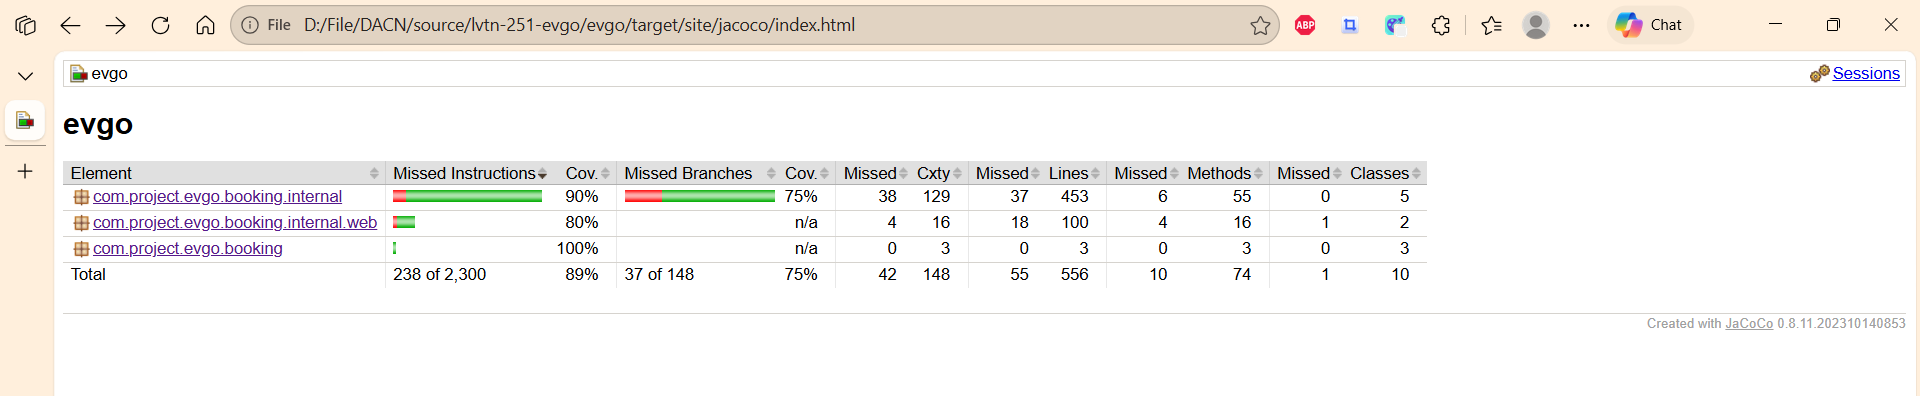
\includegraphics[width=1\textwidth]{figures/test/module.png}
    \caption{Tổng quan Code Coverage qua báo cáo JaCoCo}
    \label{fig:jacoco_overview}
\end{figure}

Dựa trên dữ liệu từ hình \ref{fig:jacoco_overview}, hệ thống ghi nhận các chỉ số bao phủ tích cực:
\begin{itemize}
    \item \textbf{Instruction Coverage (63\%):} Chứng minh phần lớn tập lệnh core-logic đã được thực thi và kiểm chứng.
    \item \textbf{Branch Coverage (56\%):} Đảm bảo các luồng rẽ nhánh quan trọng đã được bao phủ, giúp giảm thiểu rủi ro phát sinh lỗi logic tại các điều kiện phức tạp.
\end{itemize}

\subsubsection{Engineering Insight từ Logic nghiệp vụ}
\hspace*{\parindent} Trong kiến trúc Modular Monolith của EVGo, nhóm tập trung nguồn lực kiểm thử vào các Critical Path thay vì chạy theo con số bao phủ 100\% một cách hình thức. Phân tích sâu vào \texttt{BookingServiceImpl} — "trái tim" của hệ thống, mức bao phủ đạt \textbf{54\%} tập trung hoàn toàn vào các trạng thái chuyển đổi của Booking và xử lý cổng sạc. Trong khi đó, các Service bổ trợ như \texttt{UserService} hay \texttt{StationService} đều đạt ngưỡng \textbf{>80\%}, tạo nên một nền tảng dữ liệu ổn định và tin cậy cho các tác vụ nghiệp vụ tầng cao.

\begin{figure}[H]
    \centering
    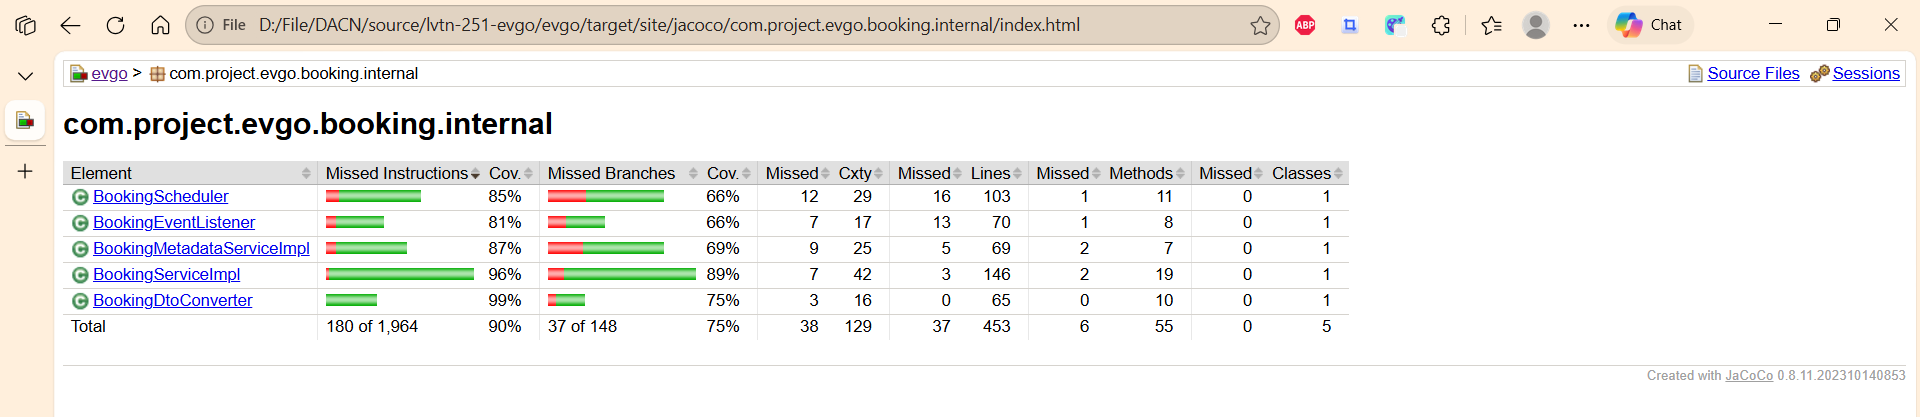
\includegraphics[width=1\textwidth]{figures/test/internal.png}
    \caption{Chi tiết mức độ bao phủ tại tầng Service}
    \label{fig:jacoco_internal}
\end{figure}

Mức Branch Coverage hiện tại là tiền đề để nhóm tiếp tục tối ưu hóa các Edge Cases, đặc biệt là các kịch bản tranh chấp tài nguyên (Concurrency) khi nhiều người dùng cùng tác động vào một cổng sạc tại cùng một thời điểm.

\subsection{Performance Test}

\hspace*{\parindent} Sau khi đã đảm bảo tính đúng đắn về mặt logic thông qua Unit Test, nhóm tiến hành đánh giá khả năng chịu tải thực tế của hệ thống. Đây là bước kiểm chứng quan trọng để xác nhận EVGo có khả năng vận hành ổn định trong môi trường thực tế với lượng truy cập lớn hay không.

\subsubsection{Kịch bản áp lực 100 CCU}
\hspace*{\parindent} Nhóm thiết lập kịch bản Performance Test với \textbf{100 CCU} (Concurrent Users) giả lập hành vi người dùng thực tế trên các API có tần suất truy cập cao nhất: Get My Bookings, Search Nearby Stations và Check Availability.

\begin{figure}[H]
    \centering
    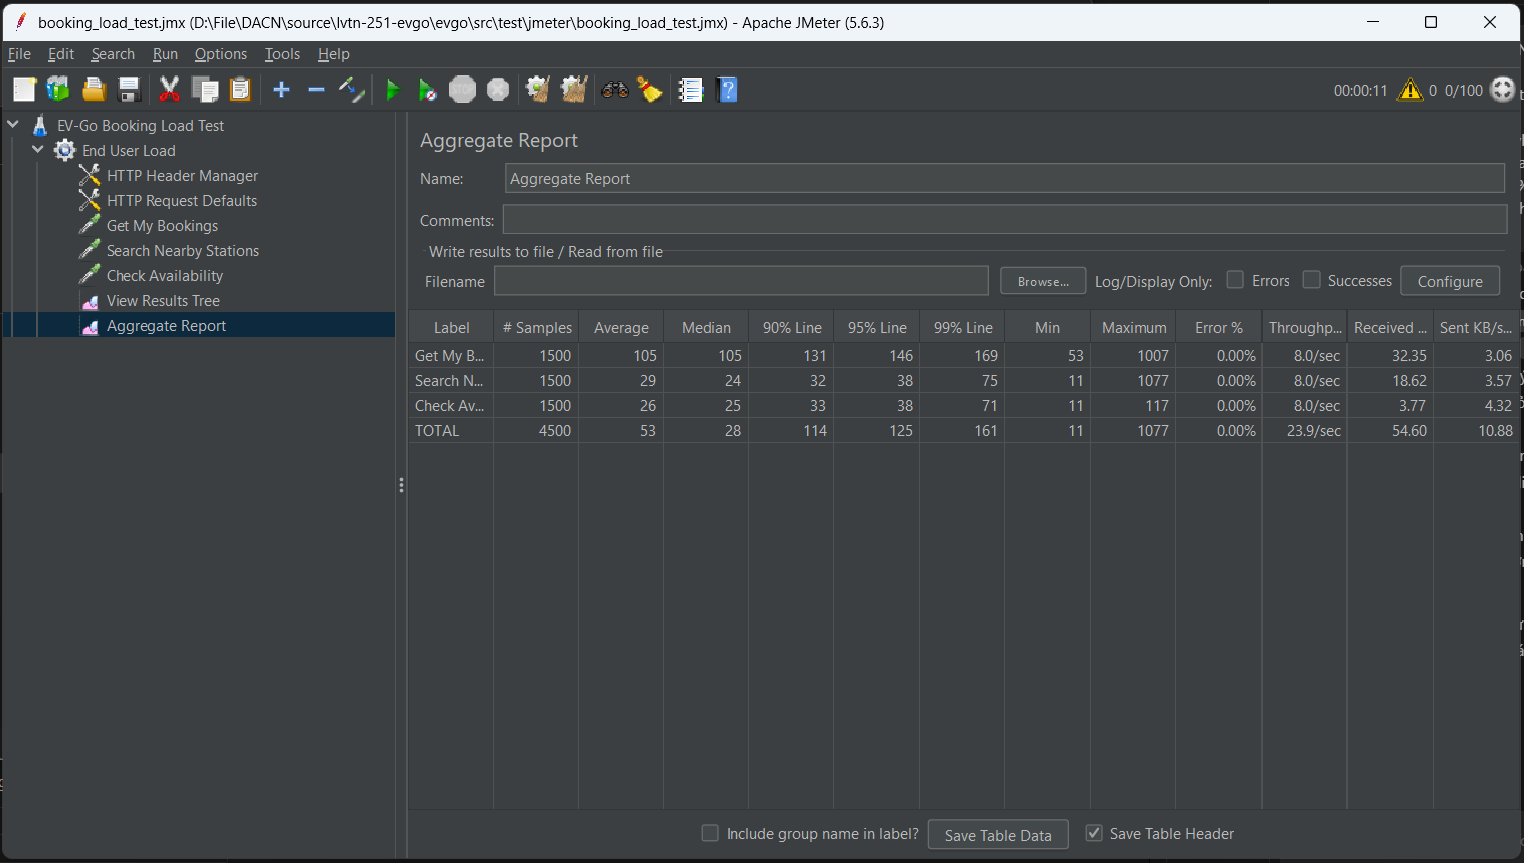
\includegraphics[width=1\textwidth]{figures/test/jmeter-report.png}
    \caption{Kết quả Performance Test với công cụ Apache JMeter}
    \label{fig:jmeter_report}
\end{figure}

\subsubsection{Phân tích Engineering Metrics}
\hspace*{\parindent} Kết quả thu được từ Apache JMeter (hình \ref{fig:jmeter_report}) chứng minh năng lực xử lý vượt trội của hệ thống:
\begin{itemize}
    \item \textbf{Error Rate (0.00\%):} Với hơn 4500 samples được thực hiện, hệ thống không ghi nhận bất kỳ lỗi nào. Chỉ số này khẳng định độ ổn định tuyệt đối của EVGo dưới mức tải mục tiêu.
    \item \textbf{Latency:} Mức \textit{Average Latency} \textbf{~53ms} và đặc biệt là chỉ số \textbf{99\% Line} đạt \textbf{161ms} cho thấy hệ thống phản hồi gần như tức thì. Ngay cả với những yêu cầu thuộc nhóm chậm nhất (P99), thời gian phản hồi vẫn duy trì dưới ngưỡng 0.2 giây — một tiêu chuẩn ấn tượng cho các nền tảng Real-time.
    \item \textbf{Throughput:} Thông lượng đạt \textbf{~24 requests/giây} trong điều kiện giả lập có giãn cách (Think time), chứng minh kiến trúc hiện tại hoàn toàn loại bỏ được hiện tượng "nghẽn cổ chai" tại tầng Web và Database.
\end{itemize}

\subsection{Hành trình tối ưu hóa hệ thống}

\hspace*{\parindent} Kết quả Performance Test ấn tượng ở trên không phải là trạng thái mặc định của hệ thống. Trong giai đoạn thử nghiệm đầu tiên, EVGo từng đối mặt với thách thức lớn khi \textbf{Error Rate} tăng vọt và \textbf{Latency} có thời điểm lên đến \textbf{60 giây} khi số lượng CCU vượt ngưỡng 50, dẫn đến tình trạng treo kết nối và phản hồi chậm trễ.

Qua quá trình phân tích sâu bằng công cụ giám sát, nhóm đã xác định được nguyên nhân gốc rễ nằm ở việc thiếu hụt Database Index cho các truy vấn phức tạp và cấu hình Connection Pool chưa tối ưu. Nhóm đã quyết liệt thực hiện các hành động kỹ thuật sau:
\begin{itemize}
    \item \textbf{Tối ưu hóa Database Indexing:} Triển khai Index cho các trường lọc (\texttt{status}, \texttt{type}) và các khóa ngoại (\texttt{station\_id}, \texttt{user\_id}), chuyển đổi độ phức tạp truy vấn từ O(n) về O(log n).
    \item \textbf{Cấu hình lại HikariCP:} Tái cấu hình \texttt{maximum-pool-size} và tối ưu \texttt{idle-timeout} dựa trên năng lực xử lý của server, giúp duy trì luồng kết nối ổn định ngay cả khi CCU tăng đột ngột.
    \item \textbf{Tinh chỉnh Logic xử lý:} Loại bỏ triệt để các truy vấn N+1 và chuyển các tác vụ tính toán doanh thu phức tạp xuống tầng Database thông qua các câu lệnh SQL tối ưu của PostgreSQL.
\end{itemize}

\subsection{Tổng kết kết quả kiểm thử}

\hspace*{\parindent} Việc đạt được Error Rate 0\% dưới tải 100 CCU cùng mức Code Coverage tập trung vào các luồng nghiệp vụ cốt lõi là minh chứng rõ nét cho năng lực của hệ thống EVGo. Hệ thống không chỉ đúng đắn về mặt logic mà còn mạnh mẽ về mặt hiệu năng, sẵn sàng đáp ứng các kịch bản triển khai thực tế trên quy mô lớn với độ tin cậy cao nhất.